\documentclass[8pt]{beamer}
\mode<presentation>
{
	\usetheme{Warsaw}
	\usecolortheme{beaver}
}

\usepackage[english]{babel}
\usepackage[utf8]{inputenc}
\usepackage[T1]{fontenc}
\usepackage{times}
\usepackage{media9}
\usepackage{color}
\usepackage{physics}
\usepackage{amsmath}
\usepackage{amsfonts}

\setbeamertemplate{caption}{\raggedright\insertcaption\par}
\setbeamerfont{caption}{size=\scriptsize}
\setlength\abovecaptionskip{-5pt}

\setbeamercolor{block title}{fg=white,bg=red!70!black}
\setbeamercolor{block body}{fg=black,bg=white!80!gray}
\setbeamercolor{itemize item}{fg=red!70!black}
\setbeamercolor{local structure}{fg=red!70!black}

\setbeamercolor{section number projected}{bg=red!70!black,fg=white}


\newtheorem*{remark}{Remark}
\newtheorem*{theor}{Theorem}

\title[\color{white}{Project N°2}]{A HIGH-ORDER DISCONTINUOUS GALERKIN METHOD FOR THE BIDOMAIN PROBLEM OF CARDIAC ELECTROPHYSIOLOGY}
\subtitle{Project N$^\circ$ 2}
\author[Federica Botta \and Matteo Calafà]{\small{\textit{Supervisors: Christian Vergara, Paola Antonietti}}\\ \vspace{4mm} Federica Botta, Matteo Calafà}
\institute[Politecnico di Milano]{\scriptsize{Course of Numerical Analysis for Partial Differential Equations}}
\date{\tiny{A.Y. 2020/2021}}


\logo{
\includegraphics[height=0.5cm]{logo_polimi.png}}



\begin{document}

\frame{\titlepage}

\begin{frame}
\frametitle{Table of Contents}
\tableofcontents
\end{frame}

\section{Introduction}
\begin{frame}
\frametitle{The physical problem}
\begin{center}
Mechanical contraction of the human heart\\

$\uparrow$

Electrical activation of the cardiac cells\\

$\downarrow$

Continuous electrical diffusion over the entire cardiac surface.\\
\end{center}
\begin{columns}
            \begin{column}{0.5\textwidth}
                  \begin{figure}[t]
                  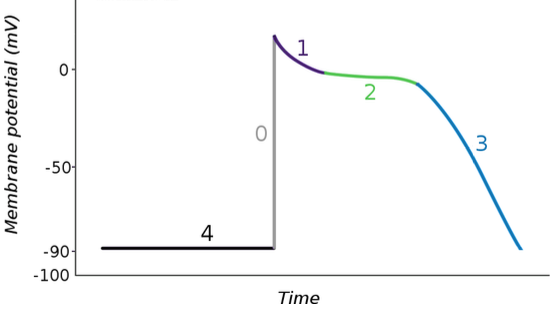
\includegraphics[width = 0.8\textwidth]{./potential_cycle.png}
                  \centering
                  \end{figure}
            \end{column}
            \begin{column}{0.5\textwidth}  
            %\begin{figure}[t]
            %      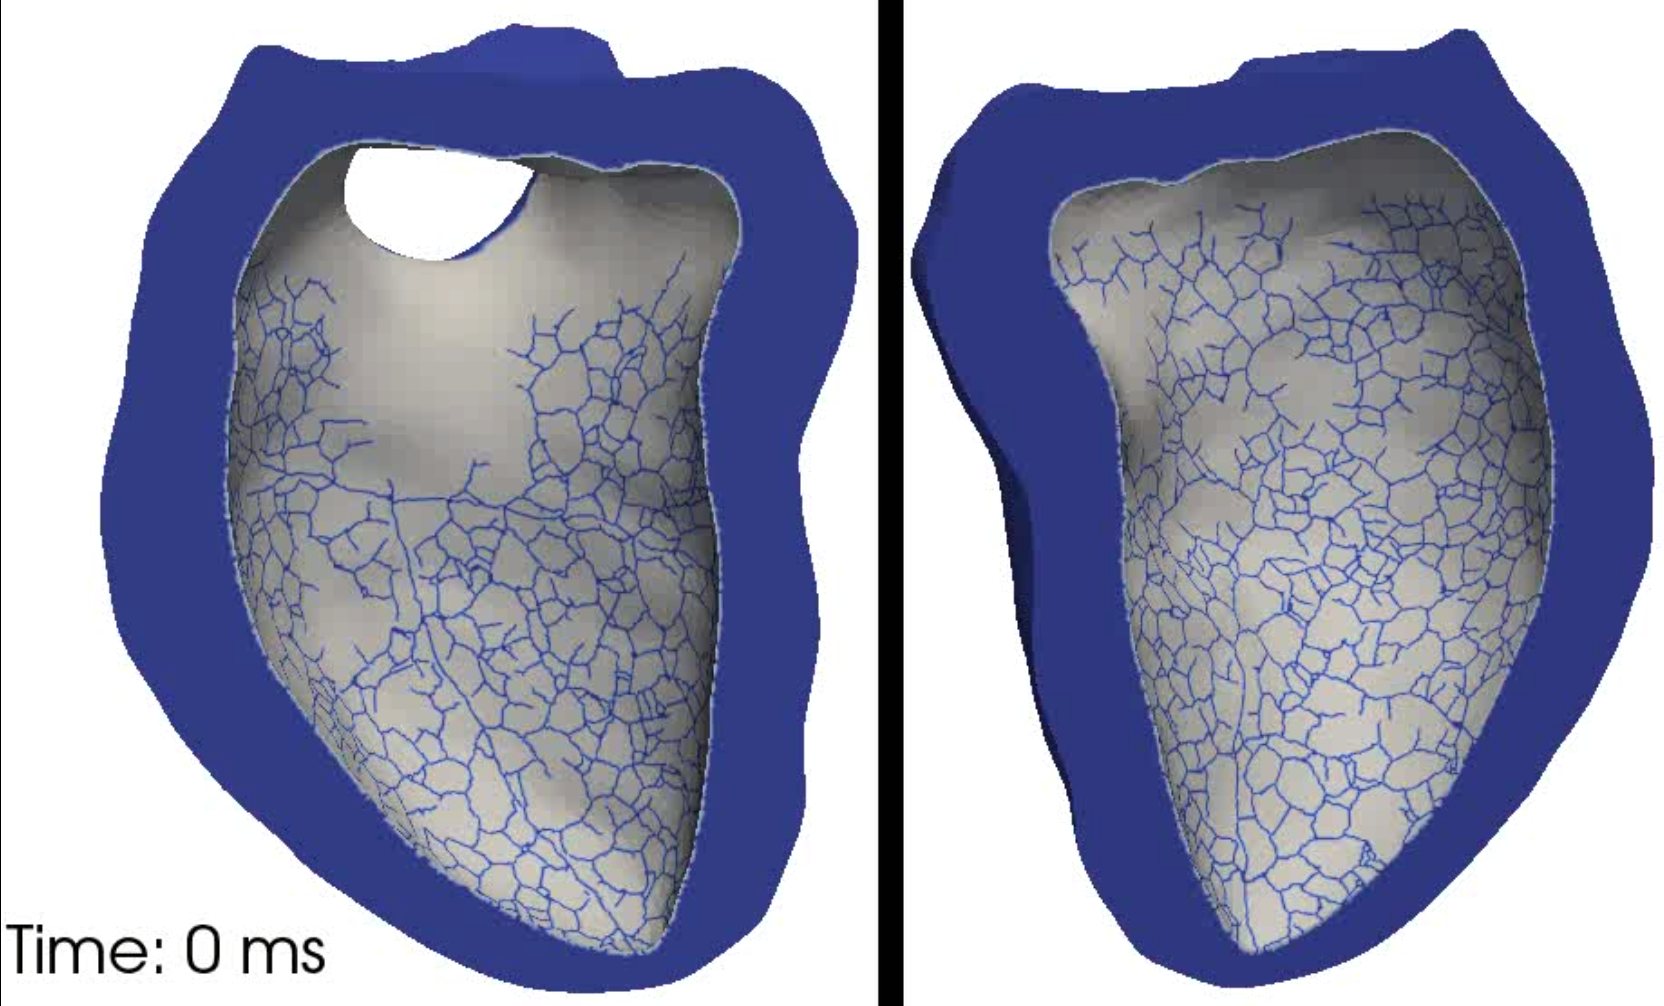
\includegraphics[width = 0.8\textwidth]{./image.png}
            %      \centering
            %      \end{figure} 
                  \includemedia[width=5cm,height=3cm,addresource=Video_Presentazione.mp4,activate=pageopen, flashvars={
                  	source=Video_Presentazione.mp4 &loop=true
                  }]{}{VPlayer.swf}
                  \centering
            \end{column}
     \end{columns}
\end{frame}


\begin{frame}
\frametitle{The mathematical model}
\center
\underline{Bidomain model + FitzHugh-Nagumo with Neumann B.C.}
\begin{equation*}
\small
\begin{cases}
\chi_m C_m\pdv{V_m}{t} - \nabla \cdot (\Sigma_i \nabla \phi_i) + \chi_m I_{ion}(V_m,w) = I_i^{ext},    & \text{in } \Omega_{mus} \cross (0,T],
\\
-\chi_m C_m\pdv{V_m}{t} - \nabla \cdot (\Sigma_e \nabla \phi_e) - \chi_m I_{ion}(V_m,w) = -I_e^{ext},    & \text{in } \Omega_{mus} \cross (0,T],
\\
I_{ion}(V_m,w)=kV_m(V_m-a)(V_m-1)+w, & \text{in } \Omega_{mus} \cross (0,T],
\\
\pdv{w}{t} = \epsilon(V_m-\gamma w),  & \text{in } \Omega_{mus} \cross (0,T],
\\
\Sigma_i\nabla \phi_i \cdot n = b_i,   & \text{on } \partial \Omega_{mus} \cross (0,T],
\\
\Sigma_e\nabla \phi_e \cdot n = b_e,   & \text{on } \partial \Omega_{mus} \cross (0,T],
\\
\text{Initial conditions for } \phi_i,\phi_e, w, & \text{in } \Omega_{mus}\cross\{t=0\}.
\end{cases}
\end{equation*}
\center \small
Unknowns: $\phi_i,\,\phi_e,\, V_m=\phi_i-\phi_e,\, w$
\end{frame}


\begin{frame}
\frametitle{Our objectives}

What had already been done:
\begin{itemize}
	\item Implementation of a Discontinuous Galerkin with FEM basis for the Bidomain problem.
	\item Implementation of a Semi-Implicit temporal scheme.
\end{itemize} \vspace{2mm}
What we did:
\begin{itemize}
	\item Implementation of a Discontinuous Galerkin with \textbf{Dubiner} basis for the Bidomain problem.
	\item Implementation of further temporal schemes.
	\item Bugs corrections and optimizations.
	\item Pseudo-realistic simulations.
\end{itemize}
\end{frame}

\section{Spacial discretization}

\subsection{Semi-discrete Discontinuous Galerkin}
\begin{frame}
	\frametitle{Discretization}
	$\qquad \qquad \qquad \qquad $ \textbf{space-dependent:} Discontinuous Galerkin method\\\vspace{2mm}
	$\qquad \qquad \qquad \qquad \nearrow$\\
	Bidomain problem\\
	$\qquad \qquad \qquad \qquad \searrow$\\\vspace{2mm}
	$\qquad \qquad \qquad \qquad $ \textbf{time-dependent:} Semi-implicit, Godunov\\ $\qquad \qquad \qquad \qquad $ operator-splitting and quasi-implicit operator-splitting
\end{frame}

\begin{frame}
	\frametitle{Semi-discrete Discontinuous Galerkin formulation}
	For any $t\in[0,T]$ find $\Phi_h(t)=[\phi_i^h(t),\phi_e^h(t)]^T \in [V_h^p]^2$  and  $w_h(t) \in V_h^p$ such that:
	\vspace{2mm}
	\begin{equation*}
	\begin{cases}
	\begin{gathered}
	\sum_{\mathcal{K} \in \tau_h} \int_{\mathcal{K}}{ \chi_m C_m \pdv{V_m^h}{t} v_h d\omega}+a_i(\phi_i^h,v_h)+\sum_{\mathcal{K} \in \tau_h} \int_{\mathcal{K}}{ \chi_m k (V_m^h-1)(V_m^h-a) V_m^h v_h d\omega}+\\
	+\sum_{\mathcal{K} \in \tau_h} \int_{\mathcal{K}}{ \chi_m w_h v_h d\omega}=(I_i^{ext},v_h), \qquad \forall v_h \in V_h^p,\\
	\end{gathered}\\
	\vspace{2mm}
	\begin{gathered}
	-\sum_{\mathcal{K} \in \tau_h} \int_{\mathcal{K}}{ \chi_m C_m \pdv{V_m^h}{t} v_h d\omega}+a_e(\phi_e^h,v_h)-\sum_{\mathcal{K} \in \tau_h} \int_{\mathcal{K}}{ \chi_m k (V_m^h-1)(V_m^h-a) V_m^h v_h d\omega}+\\
	-\sum_{\mathcal{K} \in \tau_h} \int_{\mathcal{K}}{ \chi_m w_h v_h d\omega}=(-I_e^{ext},v_h), \qquad \forall v_h \in V_h^p,\\
	\end{gathered}\\
	\vspace{2mm}
	\displaystyle \sum_{\mathcal{K} \in \tau_h} \int_{\mathcal{K}}{\pdv{w_h}{t}v_h d\omega}=\sum_{\mathcal{K} \in \tau_h} \int_{\mathcal{K}}{\epsilon (V_m^h-\gamma w_h) v_h d\omega}, \qquad \forall v_h \in V_h^p,\\
	\end{cases}
	\end{equation*}
\end{frame}
\begin{frame}
	where:
	\center
	\begin{equation*}
	\begin{aligned}
	\bullet& \quad a_l(\phi_l^h,v_h)=\sum_{\mathcal{K} \in \tau_h} \int_{\mathcal{K}}{(\Sigma_l \nabla_h \phi_k^h) \cdot \nabla_h v_h d\omega}-\sum_{F \in \mathcal{F}_h^I} \int_F { \{\{\Sigma_l \nabla_h \phi_l^h \}\} \cdot [[v_h]] d\sigma}+\\
	&-\delta \sum_{F \in \mathcal{F}_h^I} \int_F{ \{\{\Sigma_l \nabla_h v_h\}\} \cdot [[\phi_l^h]]d\sigma}+\sum_{F \in \mathcal{F}_h^I}\int_F {\Gamma [[\phi_l^h]] \cdot [[v_h]] d\sigma} \qquad l=i,e,\\
	\newline
	\bullet& \quad (I_i^{ext},v_h)=\sum_{\mathcal{K} \in \tau_h} \int_{\mathcal{K}} {I_i^{ext} v_h d\omega}+\int_{\partial \Omega}{b_i v_h d\sigma},\\
	\newline
	\bullet& \quad (-I_e^{ext},v_h)=-\sum_{\mathcal{K} \in \tau_h} \int_{\mathcal{K}} {I_e^{ext} v_h d\omega}+\int_{\partial \Omega}{b_e v_h d\sigma}.
	\end{aligned}
	\end{equation*}
\end{frame}

\subsection{Dubiner basis implementation}

\begin{frame}
\frametitle{Dubiner basis: analytical definition}
\begin{definition}[Dubiner basis] \label{dubiner}
	The Dubiner basis that generates the space $\mathbb{P}^p(\hat{K})$ of polynomials of degree $p$ over the reference triangle is the set of functions:
	\begin{equation*}
	\begin{gathered}
	 \phi_{ij}: \hat{K} \rightarrow \mathbb{R}, \\
	\phi_{ij}(\xi,\eta) =c_{ij} \, 2^j (1-\eta)^j J_i^{0,0}(\frac{2\xi}{1-\eta}-1) J_j^{2i+1,0} (2\eta-1),
	\end{gathered}
	\end{equation*}
	\vspace{2mm} \\
	\center
	for $i,j=0,\dots,p$ and $i+j \le p$, where $c_{ij} := \sqrt{\frac{2(2i+1)(i+j+1)}{4^i}}$ \\
	and $J_i^{\alpha,\beta}(\cdot)$ is the i-th Jacobi polynomial.
\end{definition}
\end{frame}

\begin{frame}
\frametitle{Properties}
\begin{itemize}
	\item They consist in a pseudo tensor-product of Jacobi polynomials if the following transformation is then applied:
	\begin{columns}
		\begin{column}{0.5\textwidth}
			\begin{equation*}\label{transformation_formula}
			\quad \quad \quad \xi=\frac{(1+a)(1-b)}{4},  \eta=\frac{(1+b)}{2}.
			\end{equation*}
		\end{column}
		\begin{column}{0.5\textwidth}  
			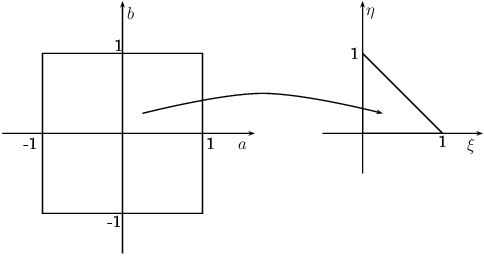
\includegraphics[width = 4cm]{./transformation.png}
		\end{column}
	\end{columns}
    \item They are $L^2(\hat{K})$ orthonormal ($\hat{K}$ is the reference triangle).
\end{itemize}
\end{frame}


\begin{frame}
\frametitle{Main works}
\begin{remark}
	Dubiner basis coefficients of a discretized function have \textbf{modal} meaning instead of a \emph{nodal} meaning.
\end{remark}
Then, our main works regarded:
\begin{itemize}
	\item Methods for the evaluation of the Dubiner functions and gradients in the reference points.
	\item Methods for the evaluation of the FEM coefficients of a discretized function starting from its Dubiner coefficients and viceversa.
	\begin{enumerate}
		\item FEM $\rightarrow$ Dubiner is needed when we use the initial solution data into the Dubiner system.
		\item FEM $\leftarrow$ Dubiner is needed when we want to get the solution obtained from the Dubiner system in a comprehensible form. 
	\end{enumerate}
\end{itemize}
\end{frame}


\begin{frame}
\frametitle{FEM-Dubiner conversion strategies}
Consider:
\begin{itemize}
	\small
	\item An element $\mathcal{K}\in \tau_h$
	\item $\{\psi_{i}\}_{i=1}^{p}$,$\{\varphi_{j}\}_{j=1}^{q}$ as the FEM and Dubiner functions with support in $\mathcal{K}$. 
	\item $\{\hat{u}_i\}_{i=1}^p$,$\{\tilde{u}_j\}_{j=1}^q$ as the FEM and Dubiner coefficients of a function $u_h$.
\end{itemize} \vspace{4mm}
\textbf{FEM $\leftarrow$ Dubiner} \\
\small Exploiting the nodal meaning of FEM, we compute its value in a point: \normalsize
\begin{equation*} \label{ref3}
\hat{u}_i = \sum_{j=1}^q \tilde{u}_j\varphi_j(x_i),
\end{equation*}
\textbf{FEM $\rightarrow$ Dubiner} \\
\small Exploiting the $L^2$-orthonormality of Dubiner, we compute its Fourier coeff.: \normalsize
\begin{equation*}\label{ref4}
\tilde{u}_j = \int_\mathcal{K} u_h(x) \varphi_j(x) \,dx = \int_{\mathcal{K}} \sum_{i=1}^p \hat{u}_i\psi_i(x) \varphi_j(x) \,dx
\end{equation*}
\end{frame}


\begin{frame}
\section{Temporal discretization}
\frametitle{Semi-implicit scheme}
Idea:
\begin{itemize}
\item treat most of the terms of the PDE implicitly,
\item treat the non-linear term semi-implictly,
\item treat the ODE implictly with the exception of the term $V_m$.
\end{itemize}
\vspace{3mm}
\begin{center}
\underline{Semi-implicit discretized system}
\end{center}
Find $\Phi^{n+1}=[\phi_i^{n+1} \phi_e^{n+1}]^T$ and $w^{n+1}$ $\forall n=0,\cdots,N-1$ such that:
\begin{equation*}
\begin{cases}
(\frac{1}{\Delta t}+\epsilon \gamma)M w^{n+1}=\epsilon M V_m^n+\frac{M}{\Delta t} w^n, \vspace{2mm} \\
(B+C_{nl}(V_m^n)) \Phi^{n+1}=r^{n+1}.
\end{cases}
\end{equation*} 
\end{frame}

\begin{frame}
\frametitle{Godunov operator-splitting scheme}
The main feature is the sub-division of the problem into two different problems to be solved sequentially, such that $L(u)=L_1(u)+L_2(u)$. In our case:
\vspace{2mm}
\begin{columns}
            \begin{column}{0.5\textwidth}
\small 1:
 \begin{equation*}
\begin{cases}
\chi_m C_m M\frac{\hat{V}_m^{n+1} - V_m^n}{\Delta t} + C(V_m^n)V_m^n +\chi_mMw^n = 0,\vspace{2mm}\\
\frac{w^{n+1}-w^n}{\Delta t} = \epsilon (V_m^n - \gamma w^n).
\end{cases}
\end{equation*}
            \end{column}
            \hspace{1cm}
            \begin{column}{0.5\textwidth}  
            \small 2:
\begin{equation*}
\begin{cases}
\chi_m C_m M\frac{V_m^{n+1} - \hat{V}_m^{n+1}}{\Delta t} + A_i\phi_i^{n+1} = F_i^{n+1}, \vspace{2mm}\\
-\chi_m C_m M\frac{V_m^{n+1} - \hat{V}_m^{n+1}}{\Delta t} + A_e\phi_e^{n+1} = F_e^{n+1}.
\end{cases}
\end{equation*}

            \end{column}
     \end{columns}
     \vspace{4mm}
\begin{center}
\underline{Godunov operator-splitting discretized system}
\end{center}
\begin{equation*}
\small
\begin{cases}
\begin{gathered}
\left(
\frac{\chi_m C_m}{\Delta t} \begin{bmatrix}M & -M \\ M & -M\end{bmatrix}
+ \begin{bmatrix} A_i & 0 \\ 0 & -A_e \end{bmatrix}
\right) \begin{bmatrix} \phi_i^{n+1} \\ \phi_e^{n+1}  \end{bmatrix} =
\begin{bmatrix} F_i^{n+1} \\ -F_e^{n+1} \end{bmatrix} + \\ -
\chi_m\begin{bmatrix} M & 0 \\ 0 & M \end{bmatrix} \begin{bmatrix} w^n \\ w^n \end{bmatrix} +
\left(\frac{\chi_mC_m}{\Delta t}\begin{bmatrix} M & 0 \\ 0 & M \end{bmatrix}
- \begin{bmatrix} C(V_m^n) & 0 \\ 0 & C(V_m^n)\end{bmatrix} 
\right) \begin{bmatrix} V_m^n \\ V_m^n \end {bmatrix},
\end{gathered} \\ \\
w^{n+1} = (1-\epsilon \gamma \Delta t) w^n + \epsilon \Delta tV_m^n.
\end{cases}
\end{equation*}

\end{frame}

\begin{frame}
\frametitle{Quasi-implicit operator-splitting scheme}
Idea:
\begin{itemize}
\item sub-division of the operator as Godunov operator-splitting
\item treat implicitly all the terms except the cubic one
\end{itemize}
\vspace{2mm}
\begin{columns}
            \begin{column}{0.5\textwidth}
\small 1:
 \begin{equation*}
\begin{cases}
\chi_m C_m M \frac{\tilde{V}_m^{n+1}-V_m^n}{\Delta t} +  C(V_m^n) V_m^{n+1} + \chi_m M w^{n+1}= 0,\vspace{2mm}\\
\frac{w^{n+1} - w^n}{\Delta t} = \epsilon (V_m^{n+1}-\gamma w^{n+1}).
\end{cases}
\end{equation*}
            \end{column}
            \hspace{1cm}
            \begin{column}{0.5\textwidth}  
            \small 2:
\begin{equation*}
\begin{cases}
\chi_m C_m M \frac{V_m^{n+1}-\tilde{V}_m^{n+1}}{\Delta t} + A_i \phi_i^{n+1}= F_i^{n+1},\vspace{2mm}\\
- \chi_m C_m M \frac{V_m^{n+1}-\tilde{V}_m^{n+1}}{\Delta t} + A_e \phi_e^{n+1}= F_e^{n+1}.
\end{cases}
\end{equation*}
            \end{column}
     \end{columns}
\vspace{3mm}
\begin{center}
\underline{Quasi-implicit operator-splitting discretized system}
\end{center}
\begin{equation*}
\quad
\begin{cases}
\left(
\begin{bmatrix} Q_n & -Q_n \\ Q_n & -Q_n \end{bmatrix} + 
\begin{bmatrix} A_i & 0 \\ 0 & -A_e\end{bmatrix}
\right)
\begin{bmatrix}
\phi_i^{n+1} \\ \phi_e^{n+1}
\end{bmatrix}
= \begin{bmatrix} R_n \\ R_n \end{bmatrix} + \begin{bmatrix} F_i^{n+1} \\  -F_e^{n+1}\end{bmatrix},\\ \\
w^{n+1} = \frac{\displaystyle w^n + \epsilon \Delta t (\phi_i^{n+1}-\phi_e^{n+1})}{\displaystyle 1+\epsilon \gamma \Delta t}.
\end{cases}
\end{equation*}
\end{frame}

\begin{frame}
\section{Uniqueness of the potentials}
\frametitle{Uniqueness}
About uniqueness of the unkowns:
\vspace{2mm}
\begin{itemize}
\item $V_m, w$ proved in \textit{Existence and uniqueness of the solution for the bidomain model used in cardiac electrophysiology} by Y. Bourgault, Y. Coudière, and C. Pierre.
\vspace{2mm}
\item $\phi_i, \phi_e$ appear only through their difference $V_m$ or their gradient. This means that there cannot be uniqueness.
\end{itemize}
\end{frame}
\begin{frame}
\frametitle{Uniqueness of potentials}
\begin{theor}
The classical solutions $\phi_i,\phi_e$ are unique up to a constant depending only on time.
\end{theor}
\begin{center}
	\textbf{STRATEGIES}
\end{center}
\begin{enumerate}
\item Imposition of the value of the function in a specific point. \\
\begin{small}
	$\phi_i(\bar{x},t) = \varphi(t) \quad \forall t \in [0,T] \quad
	\xrightarrow[]{\text{Numerical version}}\quad
	u_1^n = \varphi(t^n) \quad \forall n \in \{1,N\}$ \vspace{4mm}
\end{small}
\item Imposition of the function mean value. \\
\begin{small}
$\displaystyle \int_\Omega \phi_i\,dx = \varphi(t) \quad \forall t \in [0,T] \quad
\xrightarrow[]{\text{Numerical version}}\quad \sum_{j=1}^{N_h} u_j^n \, w_j = \varphi(t^n)\quad \forall n \in \{1,N\}$
\end{small}
\end{enumerate}
\end{frame}

\begin{frame}
\frametitle{Imposition of the value in a specific point / first coefficient}
\begin{remark}
	The aim is to impose the condition before or directly into the system to avoid ill-conditioning.
\end{remark}

\begin{equation*}
A=\begin{bmatrix}
a_{11} & a_{12} & \dots & a_{1N} \\ 
a_{21} & a_{22} & \dots & a_{2N} \\ 
a_{31} &a_{32} & \dots & a_{3N} \\
\dots & \dots & \dots & \dots \\
a_{N1}  & a_{N2} & \dots & a_{NN}
\end{bmatrix} \quad \quad \rightarrow
\quad \quad \tilde{A}=\begin{bmatrix}
1 & 0 & \dots & 0 \\ 
0 & a_{22} & \dots & a_{2N} \\ 
0 &a_{32} & \dots & a_{3N} \\
\dots & \dots & \dots & \dots \\
0  & a_{N2} & \dots & a_{NN}
\end{bmatrix}
\end{equation*}

\begin{equation*}
b=\begin{bmatrix}
b_1 \\ b_2 \\ b_3 \\ \dots \\ b_N
\end{bmatrix} \quad \rightarrow \quad
\tilde{b}=\begin{bmatrix}
c \\ b_2 -a_{21}c \\ b_3-a_{31}c \\ \dots \\ b_N-a_{N1}c
\end{bmatrix}
\quad \quad \text{($c$ is the imposed value)}
\end{equation*}
\end{frame}


\begin{frame}
\frametitle{An anaytical motivation for the mean-value imposition}
\begin{remark}
The previous strategy modifies directly the system and keeps the symmetry of the matrix. This is not possible for the mean-value imposition, we should look for a different method.
\end{remark}
\vspace{2mm}
\begin{lemma}
	The two following problems are both well-posed and have the same solution $u$, moreover $\lambda=0$.
\end{lemma}
\vspace{2mm}

\begin{columns}
	\begin{column}{0.45\textwidth}
		Find $u\in H^1(\Omega)$ such that:
		\begin{equation*}
		\begin{cases}
		\int_{\Omega}\nabla u \cdot \nabla v = \int_{\Omega} fv, \quad \forall v \in H^1(\Omega),\\[2ex]
		\int_{\Omega}u = 0.
		\end{cases}
		\end{equation*}
	\end{column}
	\begin{column}{0.55\textwidth}  
		Find $ u \in H^1(\Omega), \lambda \in \mathbb{R}$ such that:
		\begin{equation*}
		\begin{cases}
	     \int_{\Omega}\nabla u \cdot \nabla v + \lambda \int_\Omega v = \int_{\Omega} fv, \quad \forall v \in H^1(\Omega), \\[2ex]
		\int_{\Omega}u= 0.
		\end{cases}
		\end{equation*}
	\end{column}
\end{columns}
\end{frame}

\begin{frame}
\frametitle{Imposition of the mean-value}
\begin{remark}
	An equivalent formulation to the Laplace problem with Neumann B.C. and null mean has been found (the very motivation passed through the Lagrange Multipliers). We can now generalize it for the Bidomain.
\end{remark}
\begin{equation*}
A=\begin{bmatrix}
a_{11} & a_{12} & \dots & a_{1N} \\ 
a_{21} & a_{22} & \dots & a_{2N} \\ 
\dots & \dots & \dots & \dots \\
a_{N1}  & a_{N2} & \dots & a_{NN}
\end{bmatrix} \quad \quad \rightarrow
\quad \quad \tilde{A}=\begin{bmatrix}
a_{11} & a_{12} & \dots & a_{1N} & d_1\\ 
a_{21} & a_{22} & \dots & a_{2N} & d_2 \\ 
\dots & \dots & \dots & \dots & \dots \\
a_{N1}  & a_{N2} & \dots & a_{NN} & d_N \\
d_1 & d_2 & \dots & d_N & 0
\end{bmatrix}
\end{equation*}

\begin{equation*}
b=\begin{bmatrix}
b_1 \\ b_2 \\ \dots \\ b_N
\end{bmatrix} \quad \rightarrow \quad
\tilde{b}=\begin{bmatrix}
b_1 \\ b_2 \\ \dots \\ b_N \\ c
\end{bmatrix} \quad \text{($c$ is the imposed value, $ \textstyle d_i = \int_\Omega \varphi_i$)}
\end{equation*}
\end{frame}

\begin{frame}
\frametitle{Strategies choices}
Most of the times the two strategies are equivalent even if the second one is computationally more expensive. On the other hand, for very ill-posed systems, first strategy might have an overshooting effect and then a global strategy is needed. \vspace{4mm} \\
This is why we chose to adopt:
\begin{itemize}
	\item The first coefficient imposition for error analysis studies.
	\item The mean value imposition for realistic simulations (where many terms are null).
\end{itemize}
\end{frame}

\section{Numerical results}
\subsection{Error analysis}

\begin{frame}
\frametitle{Chosen data}
\begin{center}
	\begin{tabular}{|c|c|} 
		\hline 
		Domain & $\begin{bmatrix} 0 & 1 \\ 0 & 1 \end{bmatrix}$ \\
		\hline 
		$dt$ & $0.0001$ \\
		\hline
		$T$ & $0.001$ \\
		\hline
		$\chi_m$ & $10^5$ \\
		\hline
		$\Sigma_i$ & $\begin{bmatrix} 0.12 & 0 \\ 0 & 0.12 \end{bmatrix}$ \\
		\hline
		$\Sigma_e$ & $\begin{bmatrix} 0.12 & 0 \\ 0 & 0.12 \end{bmatrix}$ \\
		\hline
		$C_m$ & $10^{-2}$ \\
		\hline
		$k$ & 19.5 \\ 
		\hline
		$\varepsilon$ & 1.2 \\
		\hline
		$\gamma$ & 0.1 \\
		\hline
		$a$ & $13 \cdot 10^{-3}$ \\
		\hline
		$V_m$ exact solution & $sin(2 \pi x) sin(2 \pi y) e^{-5 t}$ \\
		\hline
		$w$ exact solution & $\frac{\varepsilon}{\varepsilon \gamma-5} sin(2 \pi x) sin(2 \pi y) e^{-5 t}$ \\
		\hline
		
	\end{tabular}
\end{center}
\end{frame}

\begin{frame}
\frametitle{Comparison between FEM and Dubiner}
\begin{columns}
	\begin{column}{0.5\textwidth}
	\begin{figure}[h]
	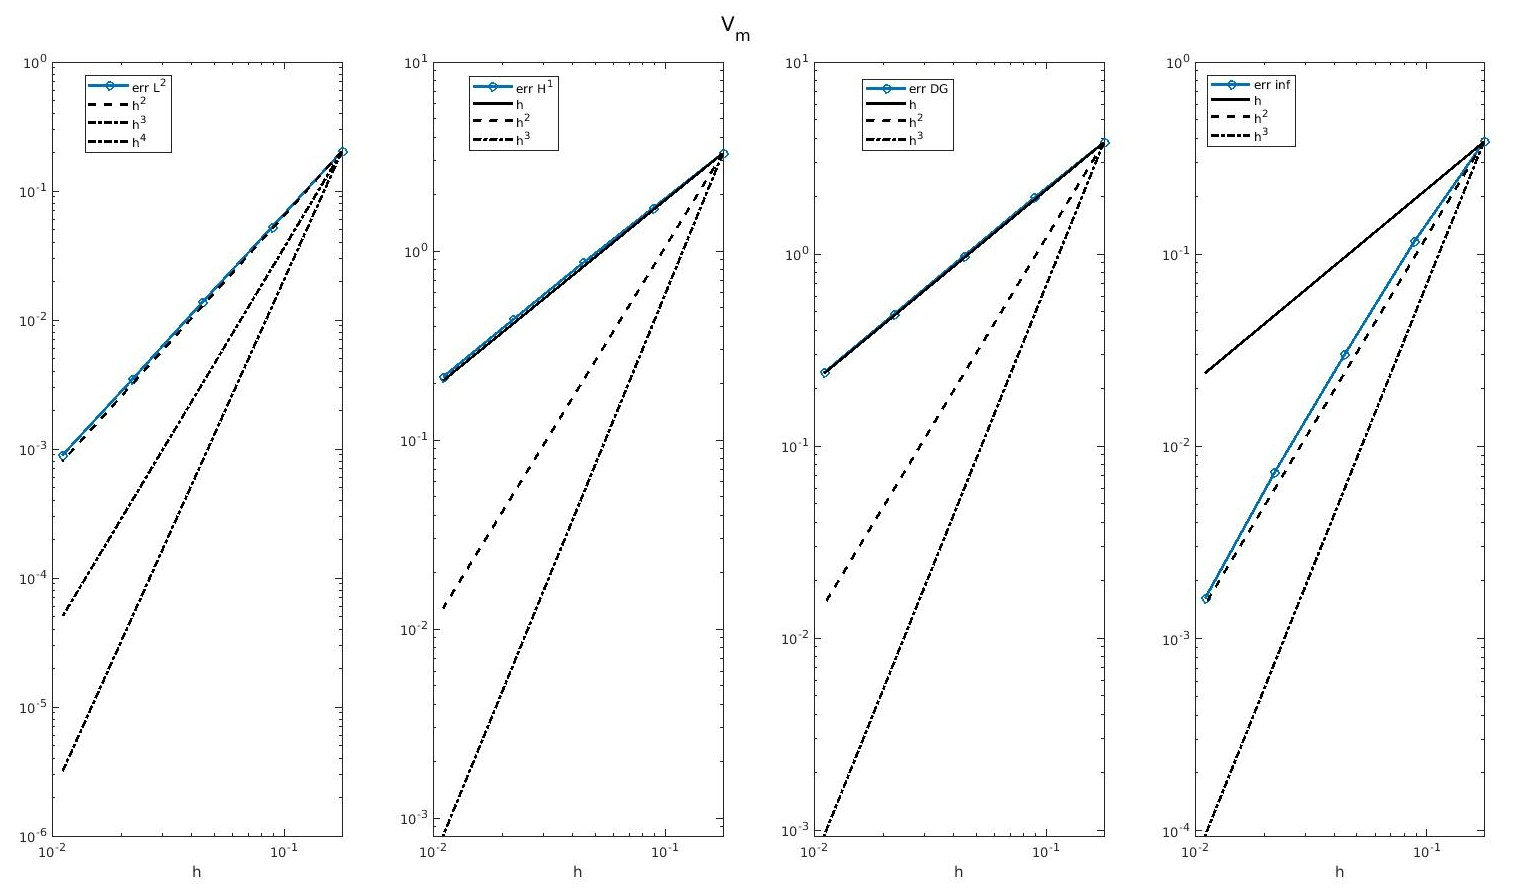
\includegraphics[width=0.8\textwidth]{D1_Vm_1.jpg} \caption{D1}
	\end{figure}
    \vspace{-4mm}
    \begin{figure}[h]
	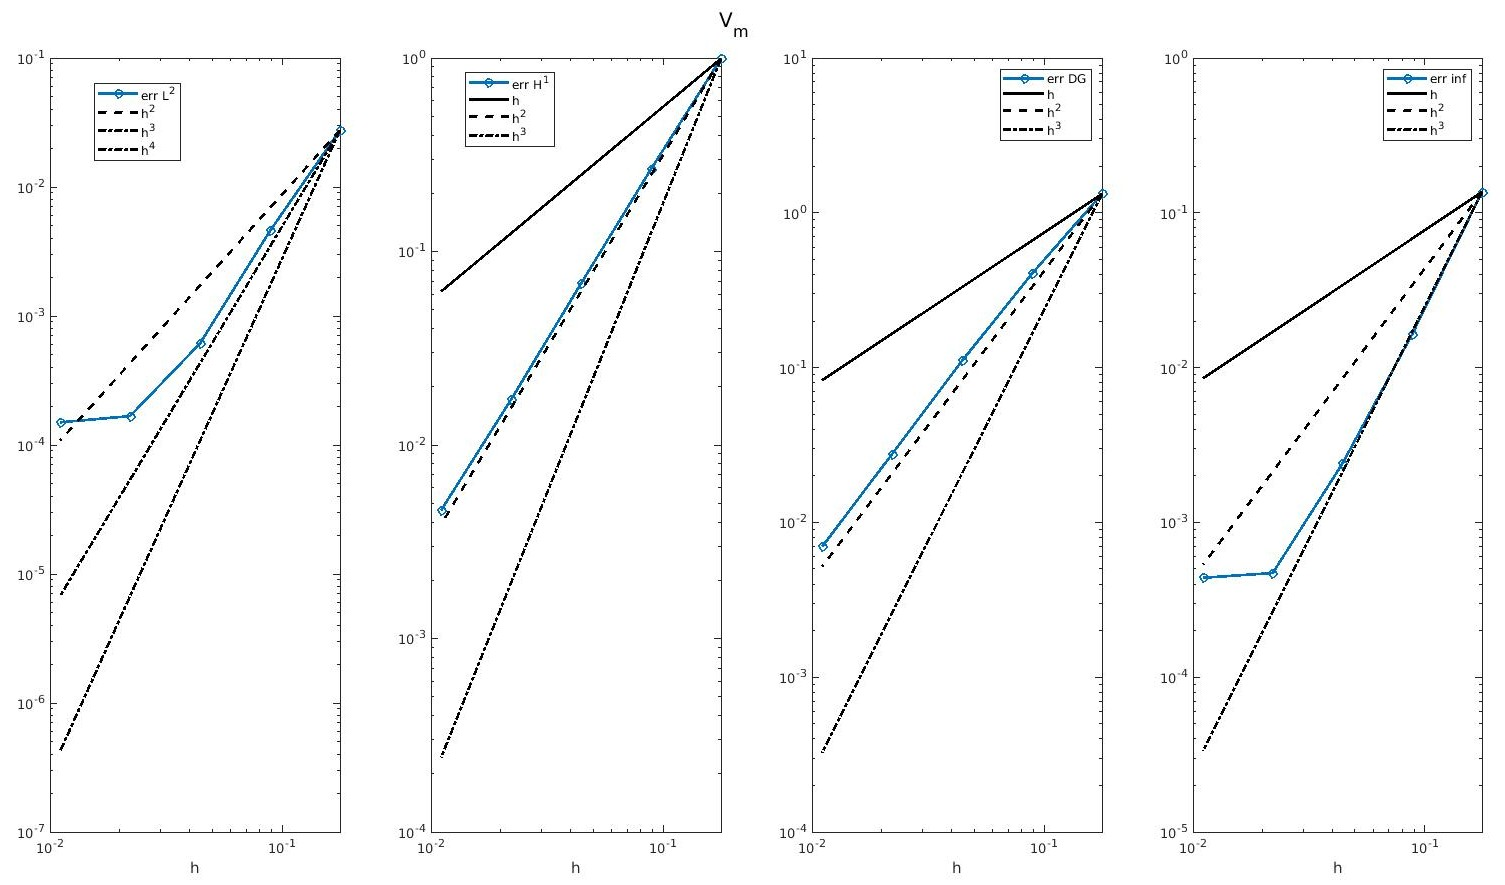
\includegraphics[width=0.8\textwidth]{D2_Vm_1.jpg} \caption{D2}
	\end{figure}
    \end{column}
    \begin{column}{0.5\textwidth}
    \begin{figure}[h]
	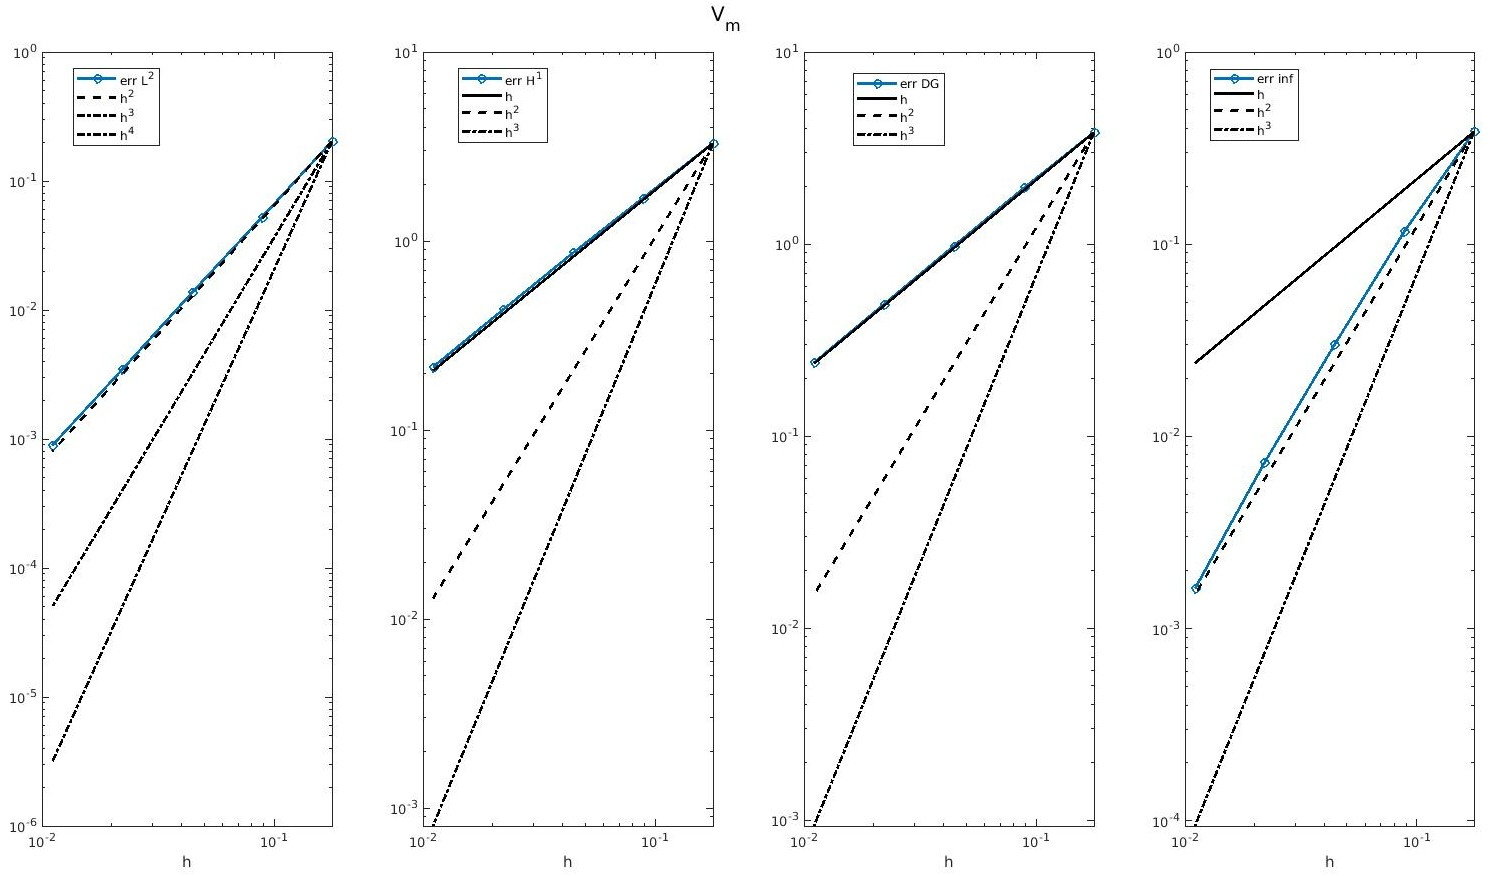
\includegraphics[width=0.8\textwidth]{P1_Vm_1.jpg} \caption{P1}
    \end{figure}
    \vspace{-4mm}
    \begin{figure}[h]
	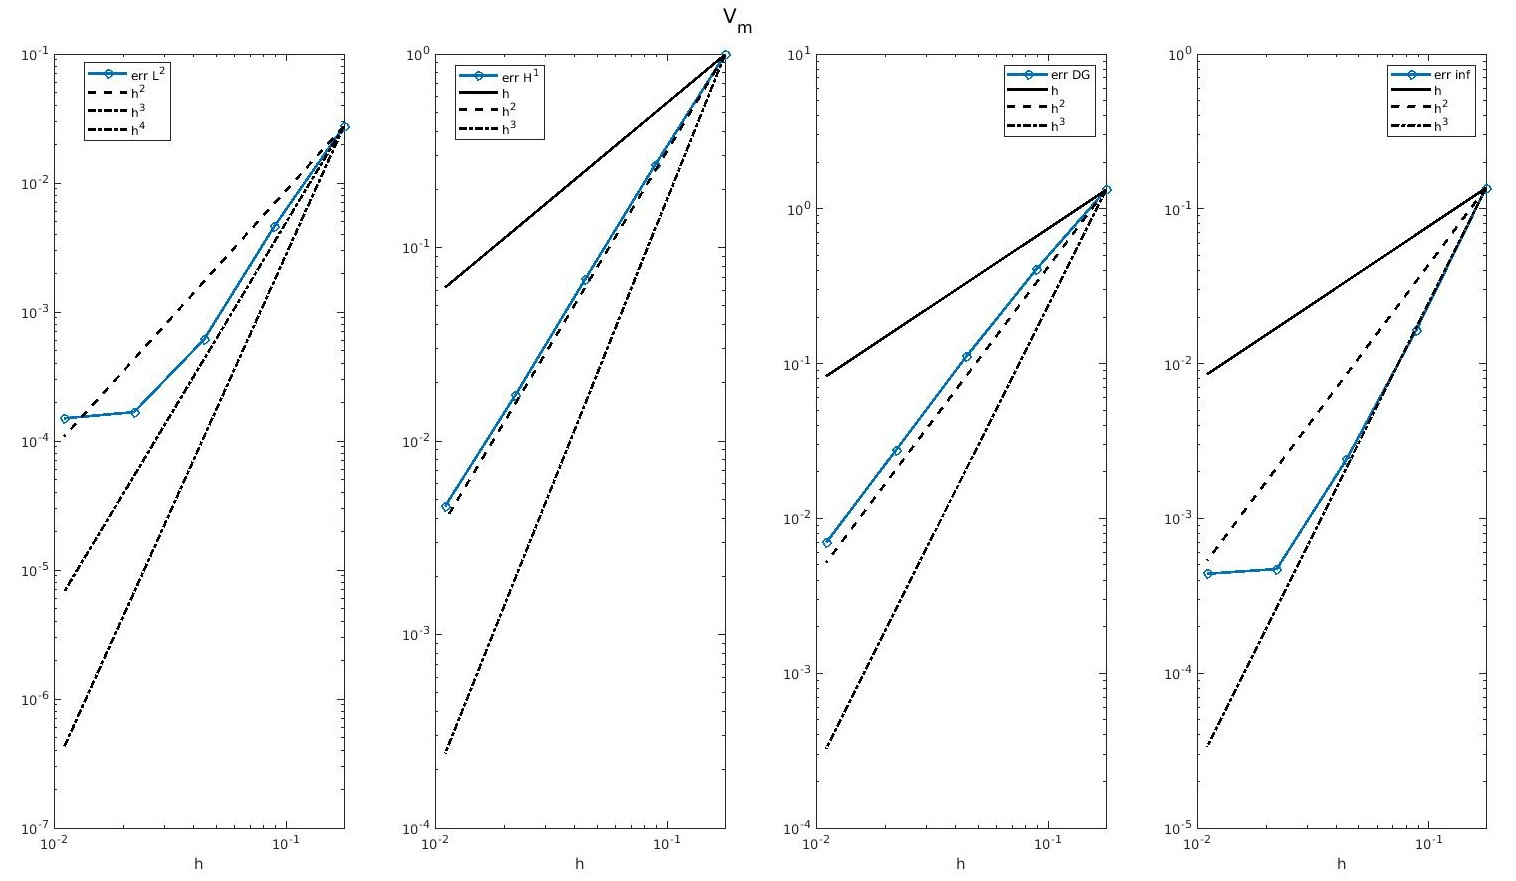
\includegraphics[width=0.8\textwidth]{P2_Vm_1.jpg} \caption{P2}
	\end{figure}
    \end{column}
\end{columns}
\end{frame}

\begin{frame}
	\frametitle{Comparison between temporal schemes}
	\begin{columns}
		\begin{column}{0.5\textwidth}
			\begin{figure}[h]
				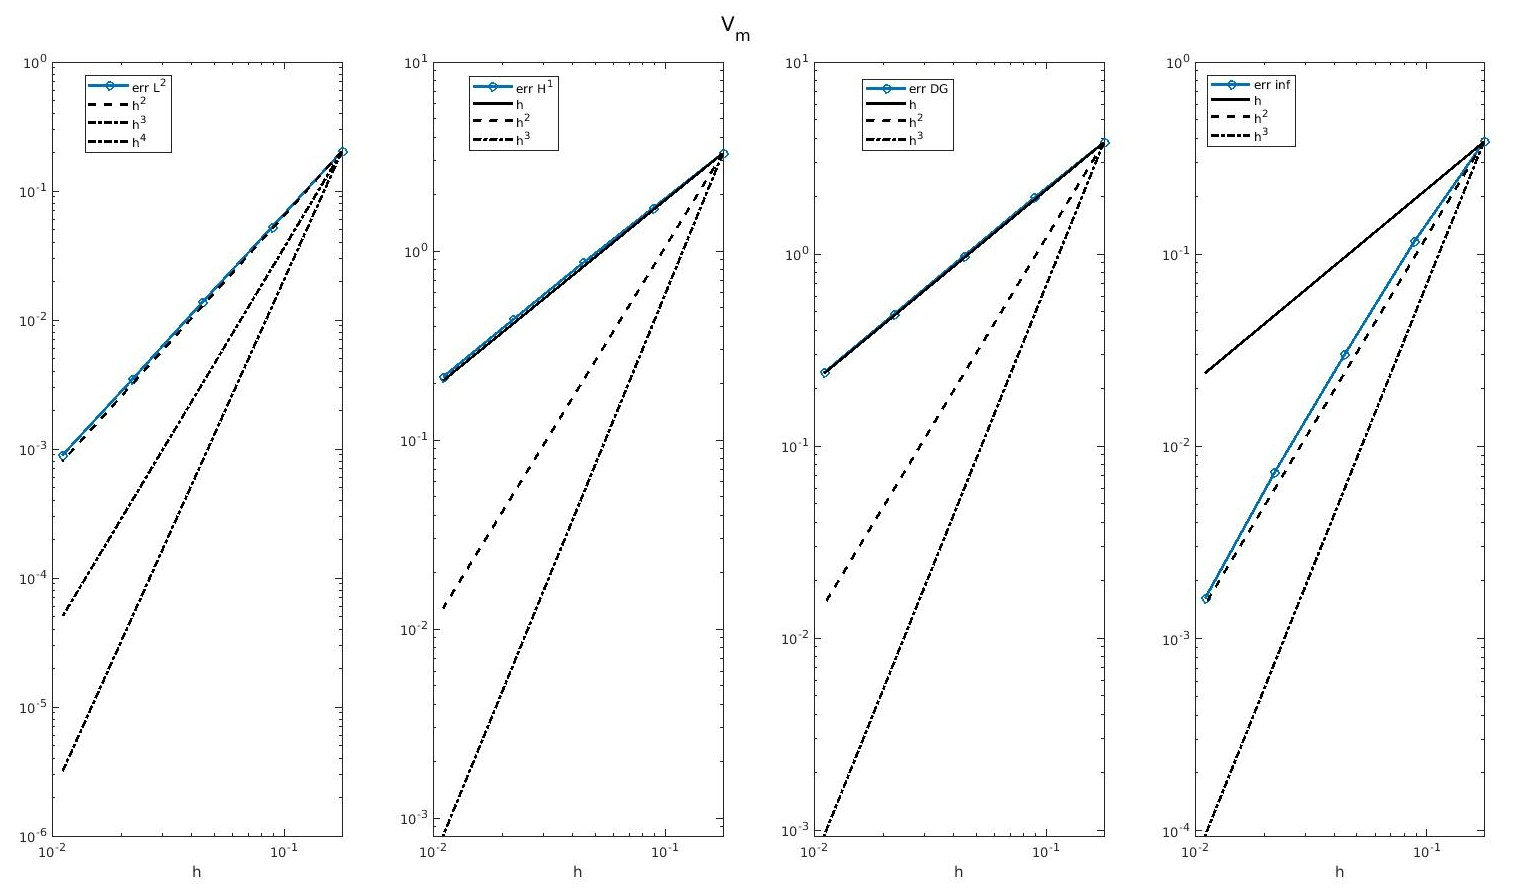
\includegraphics[width=0.8\textwidth]{D1_Vm_1.jpg} \caption{Semi-implicit}
			\end{figure}
		\end{column}
		\begin{column}{0.5\textwidth}
			\begin{figure}[h]
				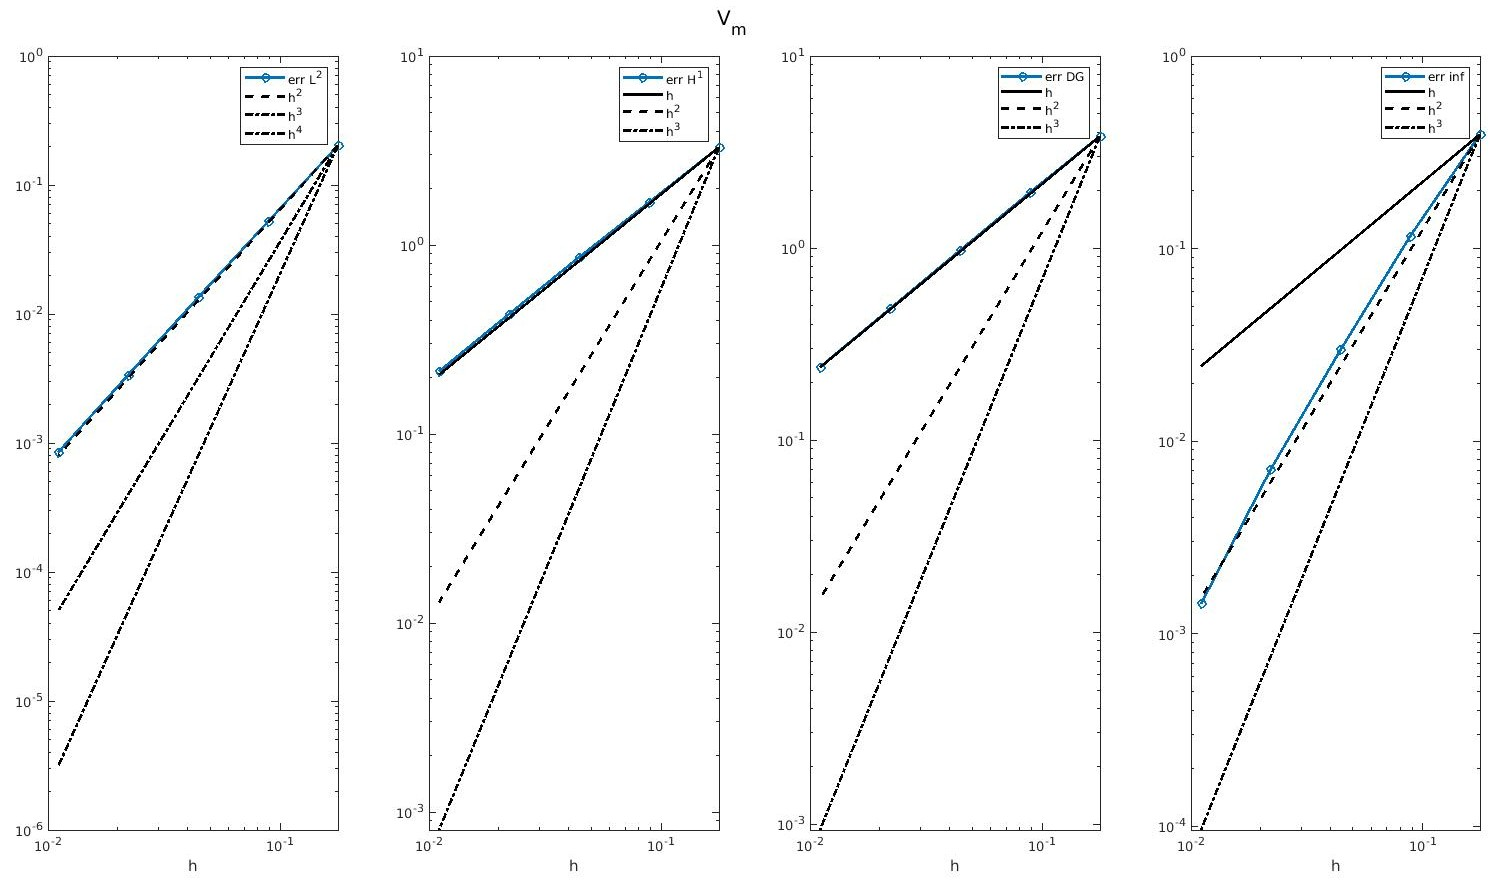
\includegraphics[width=0.8\textwidth]{D1_Vm_1_GO.jpg} \caption{Godunov OS}
			\end{figure}
		\end{column}
	\end{columns}
    \vspace{-4mm}
    \begin{figure}[h]
    	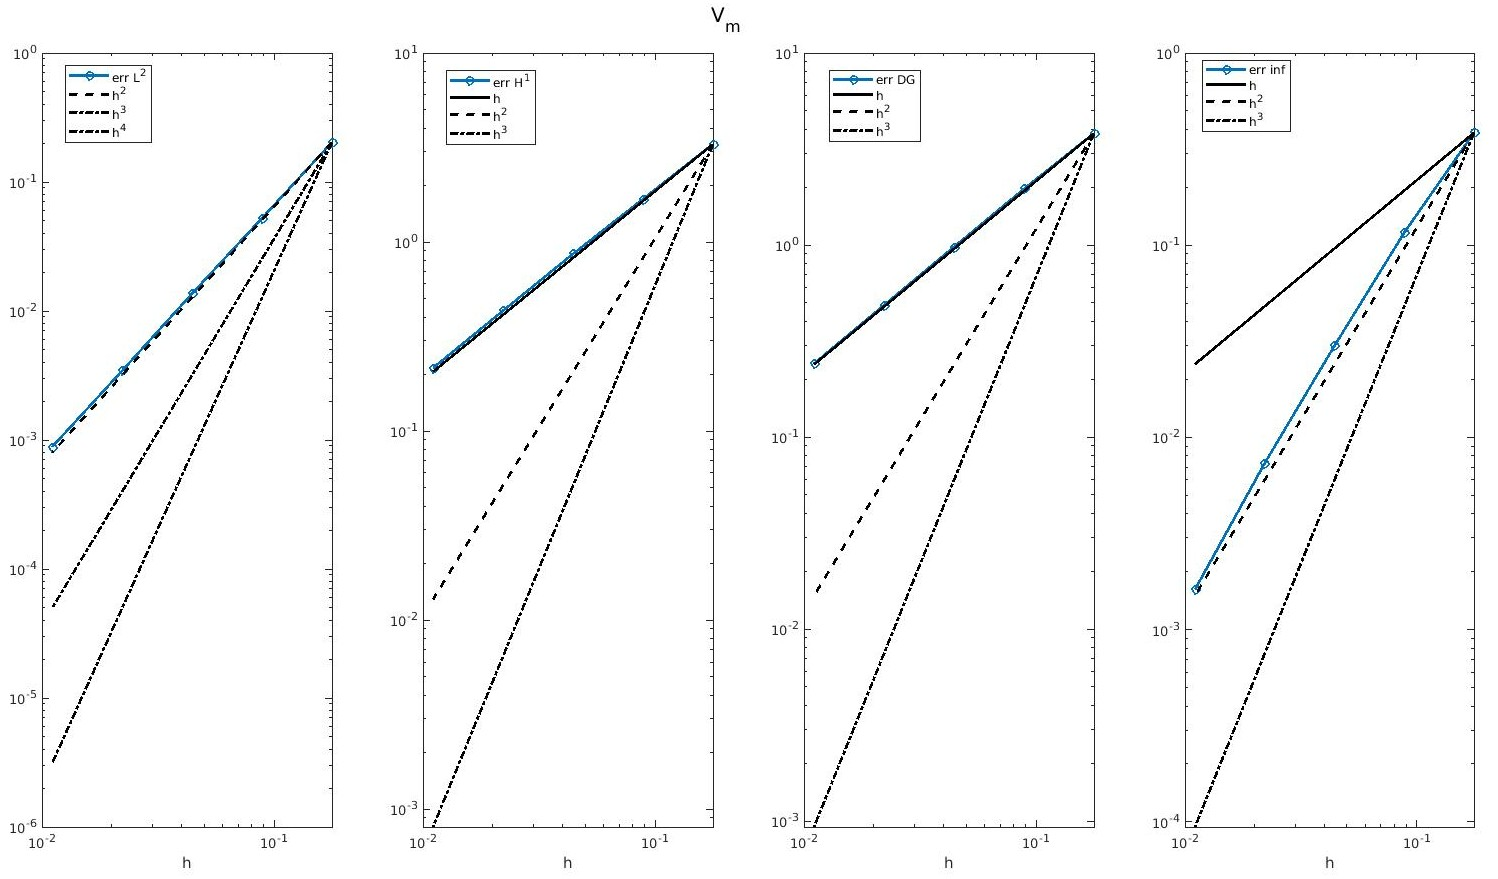
\includegraphics[width=0.4\textwidth]{D1_Vm_1_OS.jpg} \caption{Quasi-implicit OS}
    \end{figure}
\end{frame}

\begin{frame}
	\frametitle{Comparison between uniqueness imposition strategies}
	\begin{columns}
		\begin{column}{0.5\textwidth}
			\begin{figure}[h]
				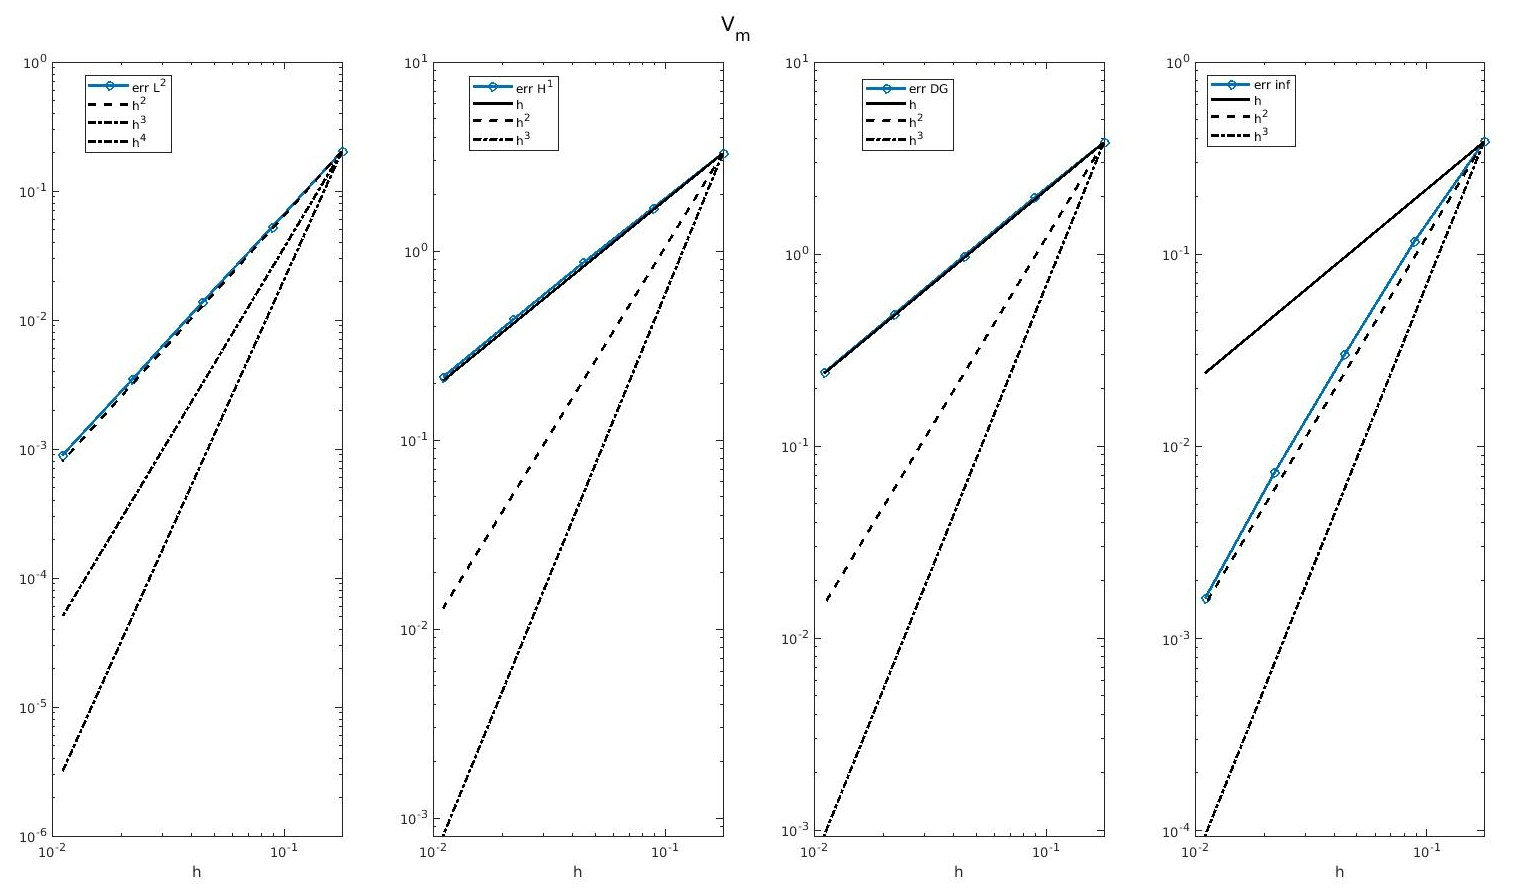
\includegraphics[width=0.8\textwidth]{D1_Vm_1.jpg} \caption{First coefficient imposition}
			\end{figure}
		\end{column}
		\begin{column}{0.5\textwidth}
			\begin{figure}[h]
				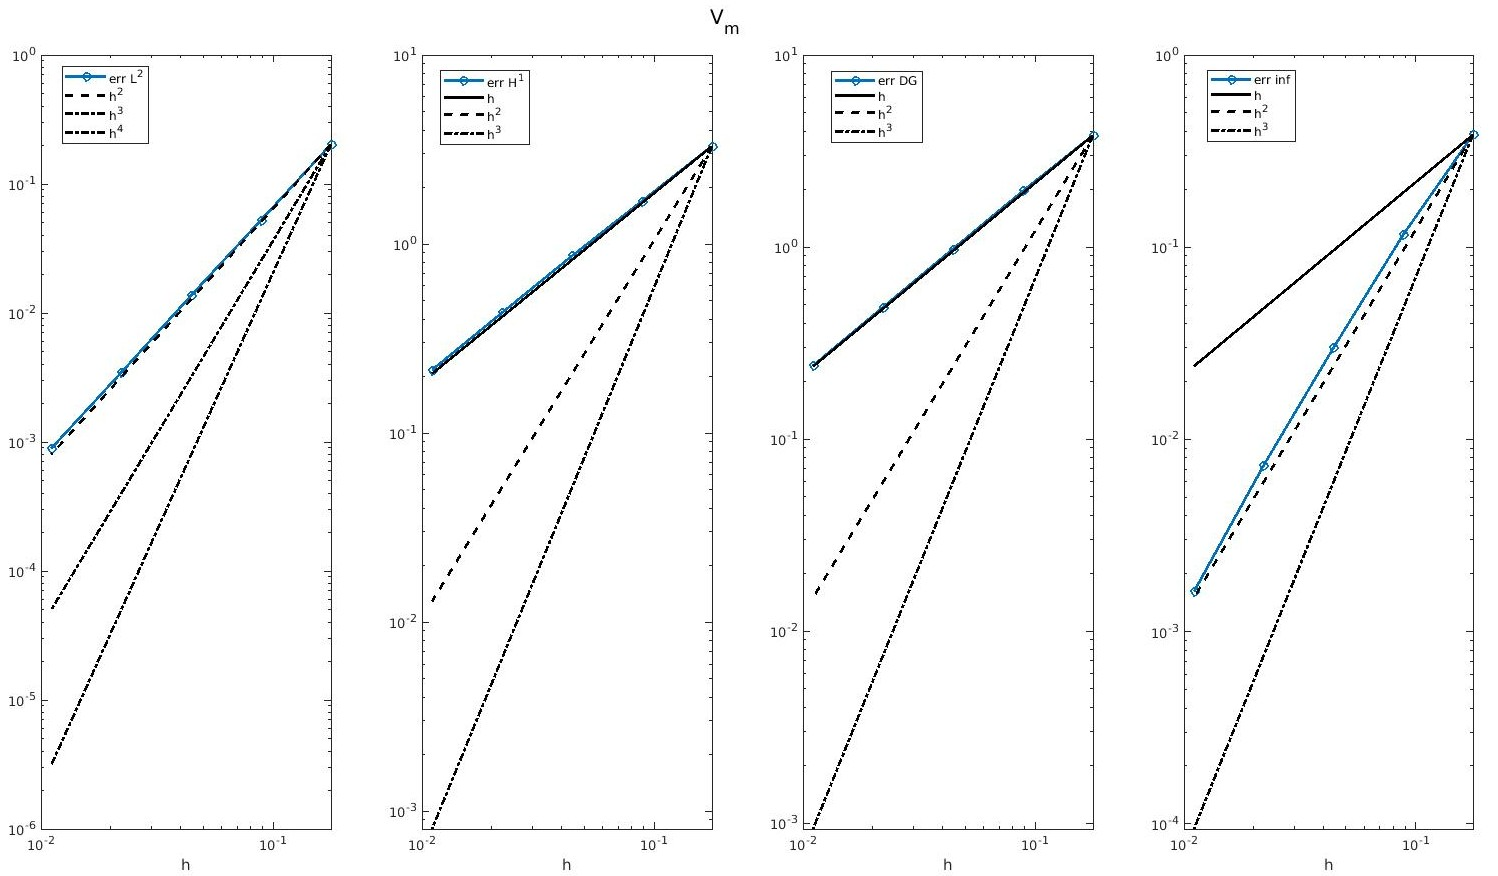
\includegraphics[width=0.8\textwidth]{D1_Vm_2.jpg} \caption{Mean value imposition}
			\end{figure}
		\end{column}
	\end{columns}
	\vspace{3mm}
	\begin{center}
	Moreover, condition number passes from $\approx 10^{17}$ to $\approx 10^7$.
	\end{center}
\end{frame}

\subsection{Toward a realistic simulation}

\begin{frame}
\frametitle{Chosen data}
\begin{center}
	\begin{tabular}{|c|c|} 
		\hline 
		Domain & $\begin{bmatrix} -0.025 & 0.035 \\ -0.025 & 0.035\end{bmatrix}$ \\
		\hline
		Initial condition for $V_m$ & 0 \\
		\hline
		Initial condition for $w$ & 0 \\
		\hline
		$I_i^{ext}$ & $I \cdot 10^3 \, \chi_{[0.001,0.002]}(t) \, \chi_{[0.0045,0.0055]}(x) \, \chi_{[0.0045,0.0055]}(y)$ \\
		\hline
		$I_e^{ext}$ & $I \cdot 10^3 \, \chi_{[0.001,0.002]}(t) \, \chi_{[0.0045,0.0055]}(x) \, \chi_{[0.0045,0.0055]}(y)$ \\
		\hline
		$b_i$ & 0 \\
		\hline
		$b_e$ & 0 \\
		\hline
		$\Sigma_i$ & $\begin{bmatrix} 0.34 & 0 \\ 0 & 0.06\end{bmatrix}$ \\
		\hline
		$\Sigma_e$ & $\begin{bmatrix} 0.62 & 0 \\ 0 & 0.24 \end{bmatrix}$ \\
		\hline 
	\end{tabular}
\end{center}
\end{frame}

\begin{frame}
	\frametitle{Missed activation, $I = 500\cdot 10^3$}
	\begin{columns}
		\begin{column}{0.25\textwidth}
			\begin{figure}[h]
				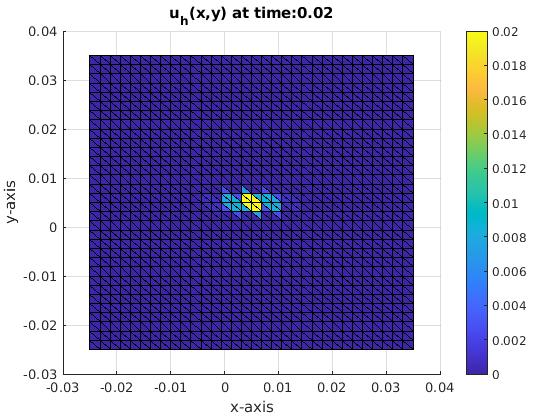
\includegraphics[width=\textwidth]{tc1-1/002.jpg}
			\end{figure}
		\end{column}
		\begin{column}{0.25\textwidth}
			\begin{figure}[h]
				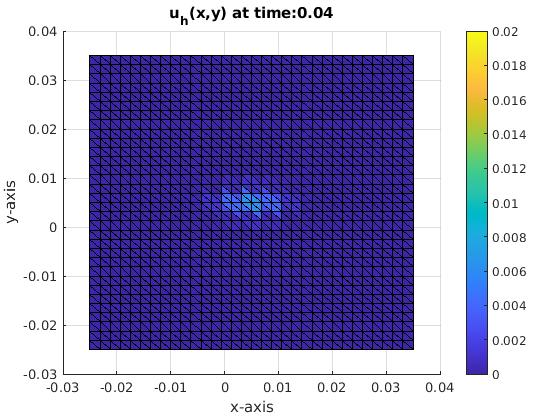
\includegraphics[width=\textwidth]{tc1-1/004.jpg}
			\end{figure}
		\end{column}
	    \begin{column}{0.25\textwidth}
		    \begin{figure}[h]
			    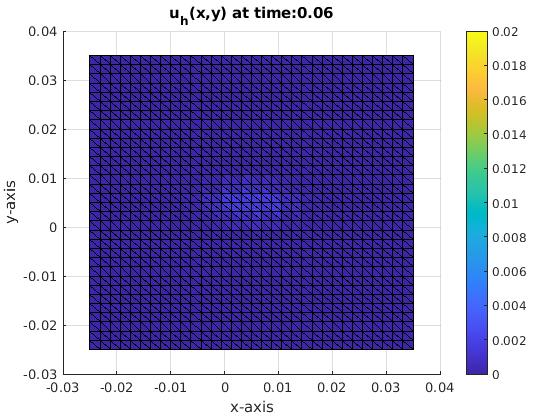
\includegraphics[width=\textwidth]{tc1-1/006.jpg}
		\end{figure}
	    \end{column}
	    \begin{column}{0.25\textwidth}
		    \begin{figure}[h]
			    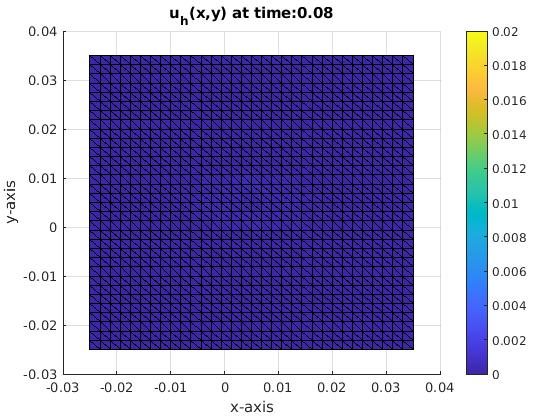
\includegraphics[width=\textwidth]{tc1-1/008.jpg}
		    \end{figure}
	\end{column}
	\end{columns}
    \begin{columns}
    	\begin{column}{0.25\textwidth}
    		\begin{figure}[h]
    			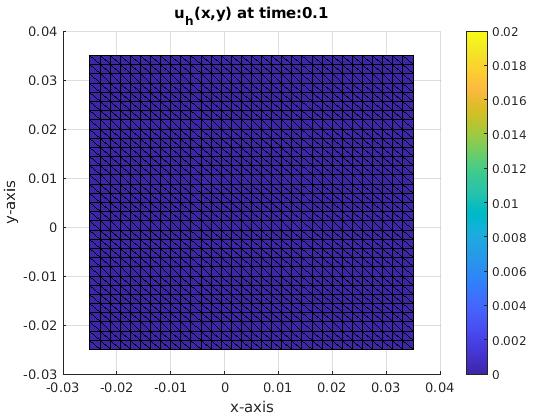
\includegraphics[width=\textwidth]{tc1-1/010.jpg}
    		\end{figure}
    	\end{column}
    	\begin{column}{0.25\textwidth}
    		\begin{figure}[h]
    			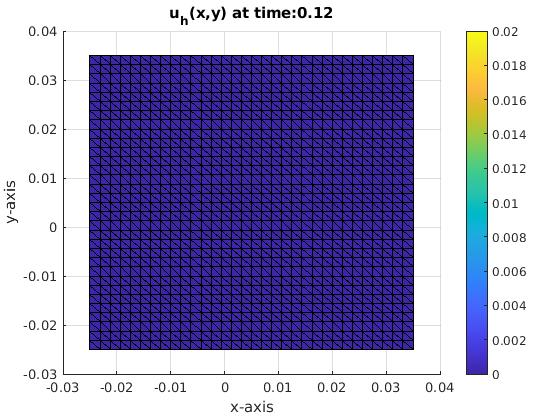
\includegraphics[width=\textwidth]{tc1-1/012.jpg}
    		\end{figure}
    	\end{column}
    	\begin{column}{0.25\textwidth}
    		\begin{figure}[h]
    			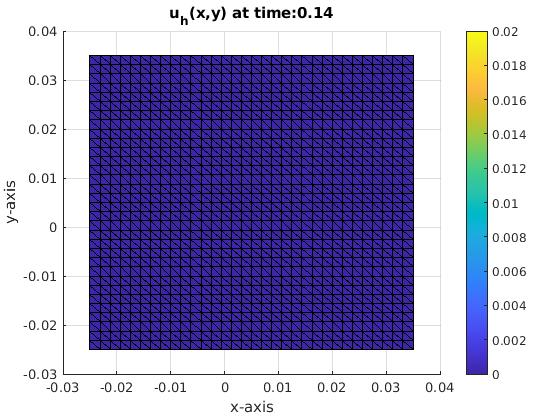
\includegraphics[width=\textwidth]{tc1-1/014.jpg}
    		\end{figure}
    	\end{column}
    	\begin{column}{0.25\textwidth}
    		\begin{figure}[h]
    			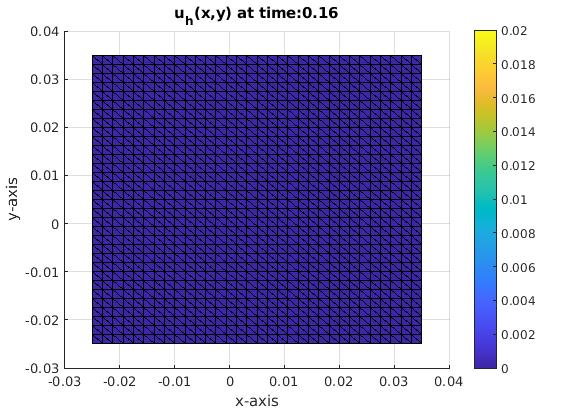
\includegraphics[width=\textwidth]{tc1-1/016.jpg}
    		\end{figure}
    	\end{column}
    \end{columns}
	\vspace{3mm}
\end{frame}

\begin{frame}
	\frametitle{Achieved activation, $I = 700\cdot 10^3$}
	\begin{columns}
		\begin{column}{0.25\textwidth}
			\begin{figure}[h]
				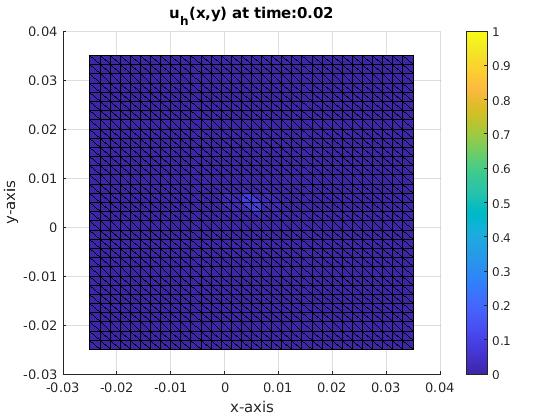
\includegraphics[width=\textwidth]{tc1-2/002.jpg}
			\end{figure}
		\end{column}
		\begin{column}{0.25\textwidth}
			\begin{figure}[h]
				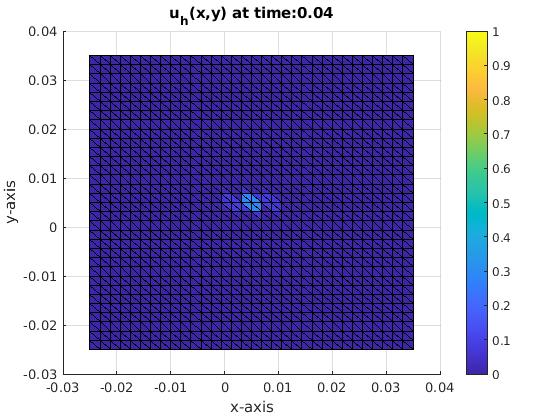
\includegraphics[width=\textwidth]{tc1-2/004.jpg}
			\end{figure}
		\end{column}
		\begin{column}{0.25\textwidth}
			\begin{figure}[h]
				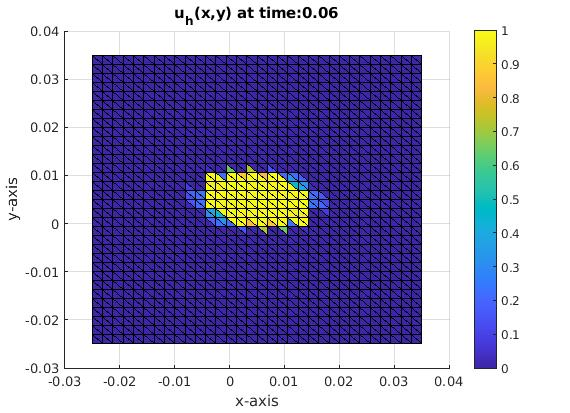
\includegraphics[width=\textwidth]{tc1-2/006.jpg}
			\end{figure}
		\end{column}
		\begin{column}{0.25\textwidth}
			\begin{figure}[h]
				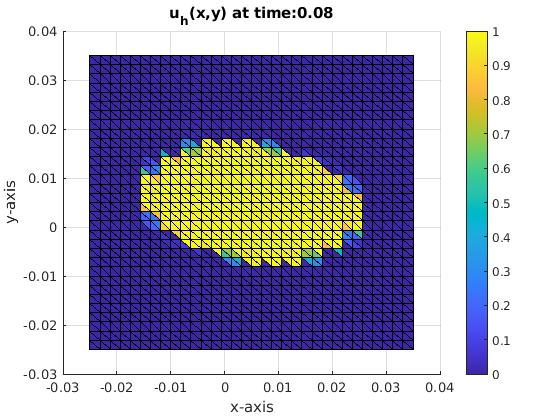
\includegraphics[width=\textwidth]{tc1-2/008.jpg}
			\end{figure}
		\end{column}
	\end{columns}
	\begin{columns}
		\begin{column}{0.25\textwidth}
			\begin{figure}[h]
				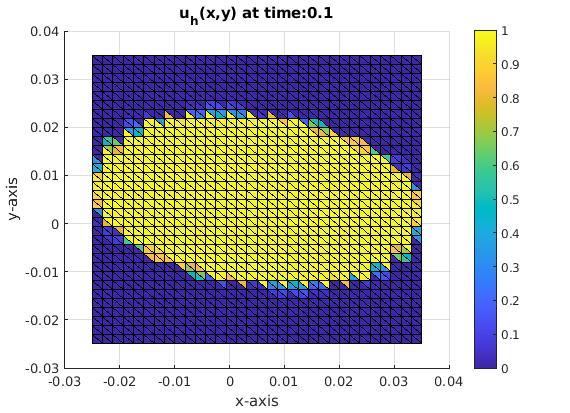
\includegraphics[width=\textwidth]{tc1-2/010.jpg}
			\end{figure}
		\end{column}
		\begin{column}{0.25\textwidth}
			\begin{figure}[h]
				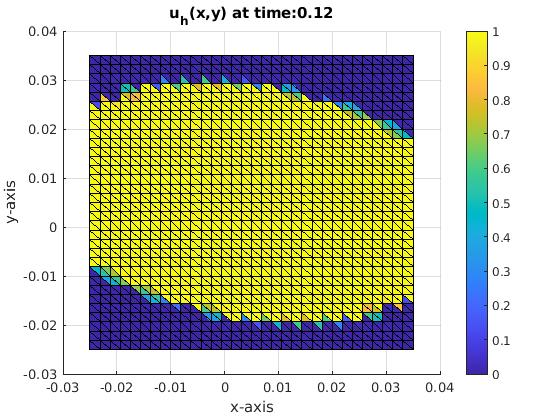
\includegraphics[width=\textwidth]{tc1-2/012.jpg}
			\end{figure}
		\end{column}
		\begin{column}{0.25\textwidth}
			\begin{figure}[h]
				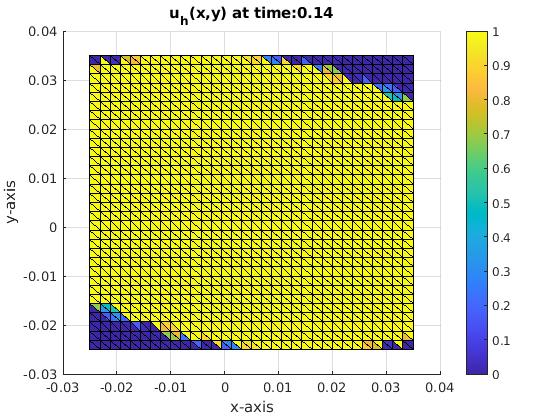
\includegraphics[width=\textwidth]{tc1-2/014.jpg}
			\end{figure}
		\end{column}
		\begin{column}{0.25\textwidth}
			\begin{figure}[h]
				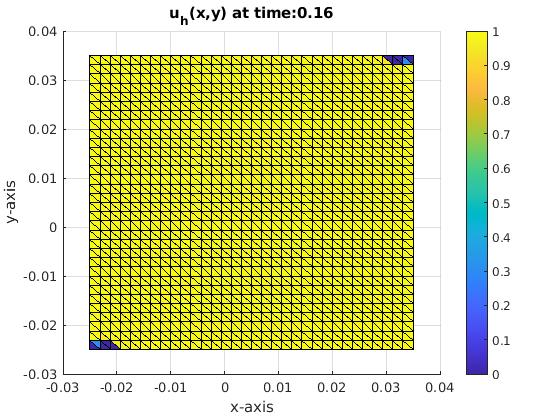
\includegraphics[width=\textwidth]{tc1-2/016.jpg}
			\end{figure}
		\end{column}
	\end{columns}
	\vspace{3mm}
\end{frame}

\begin{frame}
\frametitle{Conclusions}
\begin{itemize}
	\item Simulations truthfully represent the physical phenomenon: the threshold value for the activation, the propagation, the constant height etc.
	\item However, the rest and activation values are $0$ and $1$, different from the physiological values. Moreover, the repolarization phase misses.
This is probably due to the ionic model that is too poor and a too wide mesh. 
\end{itemize}
\vspace{4mm}
Further researches might:
\begin{itemize}
	\item Do a mesh-adaptivity study.
	\item Adopt and compare different ionic models.
\end{itemize}
\end{frame}

\end{document}
